% unit: u26
% sources: sources/085-markov-matrices-fourier-series.txt, sources/047-lecture-24-markov-matrices-fourier-series.txt, sources/203-mit18-06scf11-ses2-11sum-pdf-download-file.txt, sources/048-problem-solving-markov-matrices.txt, sources/204-mit18-06scf11-ses2-11prob-pdf-download-file.txt, sources/205-mit18-06scf11-ses2-11sol-pdf-download-file.txt, short_plan.json (s04)
\section{Markov matrices; Fourier series}\label{sec:u26}

This section gives two applications. The first uses eigenvalues: a Markov matrix moves
probabilities or populations around without creating or destroying any, and its powers
approach a steady state given by the eigenvector for $\lambda=1$. The second uses
projections: expanding a vector in an orthonormal basis is easy, and Fourier series are
exactly that expansion carried out in a space of functions.

\subsection{\texorpdfstring{\(A\)}{A} and \texorpdfstring{\(A\T\)}{its transpose} have the same eigenvalues}

\begin{proposition}[Eigenvalues of the transpose]\label{prop:u26-transpose}
For every square matrix $A$, $\det(A\T-\lambda I)=\det(A-\lambda I)$. So $A\T$ has the same
eigenvalues as $A$, with the same multiplicities.
\end{proposition}

\begin{proof}
$(A-\lambda I)\T=A\T-\lambda I$, because $I\T=I$; and a matrix and its transpose have the
same determinant (property~10, Section~\ref{sec:u20}).
\end{proof}

The eigen\emph{vectors} are usually different: an eigenvector of $A\T$ for $\lambda$ lies in
$\Nul{A\T-\lambda I}$, the left nullspace of $A-\lambda I$, not in its nullspace.

\subsection{Markov matrices}

\begin{definition}[Markov matrix]\label{def:u26-markov}
A square matrix is a \emph{Markov matrix} if every entry is nonnegative and every column
adds to $1$. With $\vb{1}=(1,1,\dots,1)$, the column condition reads $\vb{1}\T A=\vb{1}\T$.
\end{definition}

The two conditions come from probability. Entry $a_{ij}$ is the probability (or fraction of
the population) that moves from state $j$ to state $i$ in one step; probabilities are never
negative, and everything in state $j$ must go somewhere, so column $j$ adds to $1$. A
typical example is
\[
  A=\begin{bmatrix} 0.1&0.01&0.3\\ 0.2&0.99&0.3\\ 0.7&0&0.4\end{bmatrix}.
\]
Powers of a Markov matrix are Markov matrices: products of nonnegative matrices are
nonnegative, and $\vb{1}\T A^{2}=(\vb{1}\T A)A=\vb{1}\T A=\vb{1}\T$. The same computation
shows that the step $\vb{u}_{k+1}=A\vb{u}_k$ conserves the total:
$\vb{1}\T\vb{u}_{k+1}=\vb{1}\T A\vb{u}_k=\vb{1}\T\vb{u}_k$.

\begin{theorem}[Eigenvalues of a Markov matrix]\label{thm:u26-markov}
Let $A$ be a Markov matrix. Then $\lambda=1$ is an eigenvalue of $A$, and every eigenvalue
satisfies $|\lambda|\le1$.
\end{theorem}

\begin{proof}
\emph{$\lambda=1$.} Every column of $A-I$ adds to $0$, so adding all the rows of $A-I$ gives
the zero row: $\vb{1}\T(A-I)=\vb{0}\T$. The rows are dependent, so $A-I$ is singular and $1$
is an eigenvalue. (Equivalently, $A\T\vb{1}=\vb{1}$, so $\vb{1}$ is an eigenvector of $A\T$,
and Proposition~\ref{prop:u26-transpose} transfers the eigenvalue to $A$.)

\emph{$|\lambda|\le1$.} By Proposition~\ref{prop:u26-transpose} it suffices to treat $A\T$.
Let $A\T\vb{y}=\lambda\vb{y}$ with $\vb{y}\neq\vb{0}$, and choose $i$ with $|y_i|$ as large as
possible. Row $i$ of $A\T$ is column $i$ of $A$, so
\[
  |\lambda|\,|y_i|=\Bigl|\sum_j a_{ji}\,y_j\Bigr|\le\sum_j a_{ji}\,|y_j|\le|y_i|\sum_j a_{ji}=|y_i|,
\]
using $a_{ji}\ge0$ and the column sum $1$. Divide by $|y_i|>0$.
\end{proof}

The eigenvector for $\lambda=1$ is the interesting one. It is found in the nullspace of $A-I$
(not from $\vb{1}$, which lies in the left nullspace). Two more facts, which we state without
proof (they are part of the Perron--Frobenius theorem): this eigenvector can be chosen with
no negative components, and if every entry of $A$ is positive then every other eigenvalue has
$|\lambda|<1$. Zero entries can allow other eigenvalues on the unit circle: the permutation
$\left[\begin{smallmatrix} 0&1\\ 1&0\end{smallmatrix}\right]$ is a Markov matrix with
$\lambda=-1$, and its powers swap two states forever without settling down.

\begin{example}[Finding the steady-state eigenvector]\label{ex:u26-3by3}
For the $3\times3$ matrix above,
\[
  A-I=\begin{bmatrix} -0.9&0.01&0.3\\ 0.2&-0.01&0.3\\ 0.7&0&-0.6\end{bmatrix}.
\]
The last row says $0.7x_1=0.6x_3$, so try $x_1=0.6$, $x_3=0.7$. The first row then requires
$-0.54+0.01x_2+0.21=0$, so $x_2=33$. Check the middle row:
$0.12-0.33+0.21=0$. So $\vb{x}_1=(0.6,\,33,\,0.7)$, with all components positive as
promised. The middle state, which keeps $99\%$ of its contents each step, ends up holding
almost everything.
\end{example}

Now combine Theorem~\ref{thm:u26-markov} with the solution of difference equations
(Section~\ref{sec:u24}). If $A$ has independent eigenvectors, $\lambda_1=1$,
and $|\lambda_i|<1$ for $i\ge2$, then
\[
  \vb{u}_k=c_1\,1^{k}\,\vb{x}_1+c_2\lambda_2^{k}\vb{x}_2+\dots+c_n\lambda_n^{k}\vb{x}_n
  \;\longrightarrow\;c_1\vb{x}_1 .
\]
The limit is the steady state: the $\vb{x}_1$-component of the start. Because the total is
conserved, the multiple $c_1$ is fixed by $\vb{1}\T(c_1\vb{x}_1)=\vb{1}\T\vb{u}_0$. Steady states
come from $\lambda=0$ for differential equations (Section~\ref{sec:u25}) but from
$\lambda=1$ for powers.

\begin{figure}[ht]\centering
\begin{tikzpicture}[>=Stealth,node distance=4.2cm,
  st/.style={circle,draw,thick,minimum size=1.5cm,align=center}]
  \node[st] (C) {Cal.};
  \node[st,right of=C] (M) {Mass.};
  \draw[->,thick] (C) to[bend left=25] node[above] {$0.1$} (M);
  \draw[->,thick] (M) to[bend left=25] node[below] {$0.2$} (C);
  \draw[->,thick] (C) to[loop left,looseness=6] node[left] {$0.9$} (C);
  \draw[->,thick] (M) to[loop right,looseness=6] node[right] {$0.8$} (M);
  \node[right=1.6cm of M] {$A=\begin{bmatrix} 0.9&0.2\\ 0.1&0.8\end{bmatrix}$};
\end{tikzpicture}
\caption{A two-state Markov chain and its matrix. Column $j$ of $A$ lists where the
population of state $j$ goes in one year: the arrows leaving California carry $0.9$ and
$0.1$, which form column~1 and add to $1$.}
\label{fig:u26-chain}
\end{figure}

\begin{example}[California and Massachusetts]\label{ex:u26-calmass}
Each year $90\%$ of the people in California stay and $10\%$ move to Massachusetts, while
$80\%$ of Massachusetts stays and $20\%$ moves to California (Figure~\ref{fig:u26-chain}).
Start with everyone in Massachusetts:
$\vb{u}_0=(u_{\text{Cal}},u_{\text{Mass}})=(0,1000)$.

After one year $\vb{u}_1=A\vb{u}_0=1000\,(0.2,0.8)=(200,800)$. For the long run we need the
eigenvalues: $\lambda_1=1$ (Markov), and the trace $1.7$ gives $\lambda_2=0.7$ (check:
$\det A=0.72-0.02=0.7$). The eigenvectors come from
\[
  A-I=\begin{bmatrix} -0.1&0.2\\ 0.1&-0.2\end{bmatrix}\Rightarrow\vb{x}_1=(2,1),\qquad
  A-0.7I=\begin{bmatrix} 0.2&0.2\\ 0.1&0.1\end{bmatrix}\Rightarrow\vb{x}_2=(-1,1).
\]
Matching the start, $c_1(2,1)+c_2(-1,1)=(0,1000)$ gives $c_1=\tfrac{1000}{3}$ and
$c_2=\tfrac{2000}{3}$. Hence
\[
  \vb{u}_k=\frac{1000}{3}\begin{bmatrix} 2\\ 1\end{bmatrix}
  +\frac{2000}{3}(0.7)^{k}\begin{bmatrix} -1\\ 1\end{bmatrix}.
\]
At $k=1$ this gives $(\tfrac{2000-1400}{3},\tfrac{1000+1400}{3})=(200,800)$, as computed
directly; then $(340,660)$ and $(438,562)$. The populations approach
$(666\tfrac23,\,333\tfrac13)$: two thirds in California, from any start with $1000$ people.
The gap shrinks by the factor $0.7$ each year.
\end{example}

\begin{example}[The two-city model as a Markov chain]\label{ex:u26-twocity}
The matrix $A=\left[\begin{smallmatrix} 0.8&0.3\\ 0.2&0.7\end{smallmatrix}\right]$ of
the two-city example of Section~\ref{sec:u24} is a Markov matrix, which is why $\lambda_1=1$ appeared there;
$\lambda_2=1.5-1=0.5$ came from the trace. Its powers approach
\[
  A^{k}\to\begin{bmatrix} 0.6&0.6\\ 0.4&0.4\end{bmatrix}
  =\begin{bmatrix} 0.6\\ 0.4\end{bmatrix}\begin{bmatrix} 1&1\end{bmatrix},
\]
a matrix whose columns are both the steady state $(0.6,0.4)$. So
$A^{k}\vb{u}_0\to(0.6,0.4)\,(u_1+u_2)$ for every start: the long-run split does not depend on
where the 1000 people begin. Starting from $(0,1000)=(600,400)-600(1,-1)$, the first year
gives $A(0,1000)=(300,700)$, and
$\vb{u}_k=(600,400)-600(0.5)^{k}(1,-1)$ settles at $(600,400)$, the same limit as from
$(1000,0)$. Only the size of the decaying $\lambda=0.5$ part depends on the start.
\end{example}

\begin{remark}[Rows instead of columns]
Many probability texts multiply a row vector by the matrix from the left, $\vb{p}_{k+1}\T=\vb{p}_k\T P$.
Then $P=A\T$ and it is the \emph{rows} that add to $1$. Everything above holds after
transposing.
\end{remark}

\subsection{Expansion in an orthonormal basis}

Let $\vb{q}_1,\dots,\vb{q}_n$ be an orthonormal basis of $\R^{n}$. Every $\vb{v}$ is a
combination $\vb{v}=x_1\vb{q}_1+\dots+x_n\vb{q}_n$, and orthonormality makes the coefficients
trivial to find.

\begin{proposition}[Coefficients in an orthonormal basis]\label{prop:u26-coeff}
If $\vb{v}=x_1\vb{q}_1+\dots+x_n\vb{q}_n$ with orthonormal $\vb{q}_i$, then
$x_i=\vb{q}_i\T\vb{v}$. In matrix form, $Q\vb{x}=\vb{v}$ gives $\vb{x}=Q\T\vb{v}$.
\end{proposition}

\begin{proof}
Take the dot product of both sides with $\vb{q}_i$. Since $\vb{q}_i\T\vb{q}_j=0$ for $j\neq i$
and $\vb{q}_i\T\vb{q}_i=1$, every term on the right vanishes except
$x_i\vb{q}_i\T\vb{q}_i=x_i$. In matrix language, $Q$ is square with orthonormal columns, so
$Q^{-1}=Q\T$ (Section~\ref{sec:u19}), and row $i$ of $Q\T\vb{v}$ is $\vb{q}_i\T\vb{v}$.
\end{proof}

Each term $x_i\vb{q}_i=(\vb{q}_i\T\vb{v})\vb{q}_i$ is the projection of $\vb{v}$ onto the line
through $\vb{q}_i$, so the expansion writes $\vb{v}$ as the sum of its projections onto $n$
perpendicular lines. For instance, with $\vb{q}_1=(1,1)/\sqrt2$ and $\vb{q}_2=(1,-1)/\sqrt2$,
the vector $\vb{v}=(3,1)$ has $x_1=4/\sqrt2=2\sqrt2$ and $x_2=2/\sqrt2=\sqrt2$, and indeed
$2\sqrt2\,\vb{q}_1+\sqrt2\,\vb{q}_2=(2,2)+(1,-1)=(3,1)$. No linear system had to be solved.

\subsection{Fourier series: orthogonal functions}

Fourier's idea was to do the same thing with functions. A periodic function
$f(x)=f(x+2\pi)$ is to be written as
\[
  f(x)=a_0+a_1\cos x+b_1\sin x+a_2\cos2x+b_2\sin2x+\cdots .
\]
The ``vectors'' are now functions, and the basis $1,\cos x,\sin x,\cos2x,\sin2x,\dots$ is
infinite: we have moved to an infinite-dimensional vector space. To speak of orthogonality
we need an inner product. For vectors, $\vb{v}\T\vb{w}=v_1w_1+\dots+v_nw_n$ multiplies
components and adds. A function has a continuum of ``components'' $f(x)$, so we multiply
values and integrate over one period:
\[
  (f,g)=\int_{0}^{2\pi}f(x)\,g(x)\,dx,\qquad \|f\|^{2}=\int_{0}^{2\pi}f(x)^{2}\,dx .
\]

\begin{proposition}[The Fourier basis is orthogonal]\label{prop:u26-orth}
The functions $1,\cos x,\sin x,\cos2x,\sin2x,\dots$ are orthogonal for this inner product,
and $\|1\|^{2}=2\pi$, $\|\cos kx\|^{2}=\|\sin kx\|^{2}=\pi$ for $k\ge1$.
\end{proposition}

\begin{proof}
For an integer $m\neq0$, $\int_0^{2\pi}\cos mx\,dx=\int_0^{2\pi}\sin mx\,dx=0$, since each is
a whole number of periods. The product formulas
\begin{align*}
  \cos jx\cos kx&=\tfrac12[\cos(j-k)x+\cos(j+k)x],\\
  \sin jx\sin kx&=\tfrac12[\cos(j-k)x-\cos(j+k)x],\\
  \sin jx\cos kx&=\tfrac12[\sin(j+k)x+\sin(j-k)x]
\end{align*}
turn every product of two different basis functions into such terms, so its integral is
$0$. (For example $\int_0^{2\pi}\sin x\cos x\,dx=\bigl[\tfrac12\sin^{2}x\bigr]_0^{2\pi}=0$.) When
$j=k\ge1$, $\cos^{2}kx=\tfrac12(1+\cos2kx)$ and $\sin^{2}kx=\tfrac12(1-\cos2kx)$ integrate to
$\pi$, and $\int_0^{2\pi}1\,dx=2\pi$.
\end{proof}

\begin{theorem}[Fourier coefficients]\label{thm:u26-fourier}
If $f(x)=a_0+\sum_{k\ge1}(a_k\cos kx+b_k\sin kx)$, then
\[
  a_0=\frac{1}{2\pi}\int_0^{2\pi}f(x)\,dx,\qquad
  a_k=\frac1\pi\int_0^{2\pi}f(x)\cos kx\,dx,\qquad
  b_k=\frac1\pi\int_0^{2\pi}f(x)\sin kx\,dx .
\]
\end{theorem}

\begin{proof}
Exactly as in Proposition~\ref{prop:u26-coeff}: take the inner product of both sides with
$\cos kx$, that is, multiply by $\cos kx$ and integrate from $0$ to $2\pi$. By
Proposition~\ref{prop:u26-orth} every term on the right integrates to zero except
$a_k\int_0^{2\pi}\cos^{2}kx\,dx=\pi a_k$. Dividing by $\pi$ gives $a_k$; the same steps with
$\sin kx$ give $b_k$, and with the constant $1$ (whose squared length is $2\pi$) give $a_0$.
(We integrate the infinite sum term by term; for the functions met in practice this is
justified, and the series then converges to $f(x)$ wherever $f$ is continuous.)
\end{proof}

Each coefficient is a projection: $a_k=(f,\cos kx)/(\cos kx,\cos kx)$ is the formula
$\vb{a}\T\vb{b}/\vb{a}\T\vb{a}$ for projecting $\vb{b}$ onto the line through $\vb{a}$
(Section~\ref{sec:u17}), with functions in place of vectors. The basis is orthogonal but not
orthonormal, which is why we divide by $\pi$ or $2\pi$. In particular, $a_0$ is the average
value of $f$.

\begin{example}[A square wave]\label{ex:u26-square}
Let $f(x)=1$ for $0<x<\pi$ and $f(x)=-1$ for $\pi<x<2\pi$, extended with period $2\pi$. Its
average is $0$, so $a_0=0$. For $k\ge1$,
\[
  a_k=\frac1\pi\Bigl(\int_0^{\pi}\cos kx\,dx-\int_\pi^{2\pi}\cos kx\,dx\Bigr)=\frac1\pi(0-0)=0,
\]
\[
  b_k=\frac1\pi\Bigl(\int_0^{\pi}\sin kx\,dx-\int_\pi^{2\pi}\sin kx\,dx\Bigr)
  =\frac1\pi\Bigl(\frac{1-\cos k\pi}{k}-\frac{\cos k\pi-1}{k}\Bigr)
  =\frac{2\,(1-(-1)^{k})}{\pi k}.
\]
So $b_k=4/(\pi k)$ for odd $k$ and $b_k=0$ for even $k$:
\[
  f(x)=\frac4\pi\Bigl(\sin x+\frac{\sin3x}{3}+\frac{\sin5x}{5}+\cdots\Bigr).
\]
Only sines appear because $f$ is odd about $x=\pi$, like the sines. At $x=\pi/2$, where
$f=1$, the series gives $1=\tfrac4\pi\bigl(1-\tfrac13+\tfrac15-\cdots\bigr)$, which is Leibniz's
formula $\tfrac\pi4=1-\tfrac13+\tfrac15-\cdots$. Figure~\ref{fig:u26-square} shows partial
sums approaching the square wave.
\end{example}

\begin{figure}[ht]\centering
\begin{tikzpicture}
\begin{axis}[width=0.72\textwidth,height=0.36\textwidth,xmin=0,xmax=6.2832,ymin=-1.45,ymax=1.45,
  axis lines=left,xtick={0,1.5708,3.1416,4.7124,6.2832},
  xticklabels={$0$,$\tfrac\pi2$,$\pi$,$\tfrac{3\pi}2$,$2\pi$},ytick={-1,1},
  extra y ticks={0},extra y tick style={grid=major,grid style={gray!50}},
  every axis plot/.append style={samples=200,domain=0:6.2832},
  legend style={draw=none,font=\small,at={(1.02,0.5)},anchor=west},legend cell align=left]
  \addplot[black,very thick,domain=0:3.1416,samples=2] {1};
  \addlegendentry{$f$}
  \addplot[black,very thick,domain=3.1416:6.2832,samples=2,forget plot] {-1};
  \addplot[blue!70,thick] {4/pi*sin(deg(x))};
  \addlegendentry{1 term}
  \addplot[orange!90!black,thick] {4/pi*(sin(deg(x))+sin(deg(3*x))/3)};
  \addlegendentry{2 terms}
  \addplot[red!80!black,thick] {4/pi*(sin(deg(x))+sin(deg(3*x))/3+sin(deg(5*x))/5+sin(deg(7*x))/7+sin(deg(9*x))/9)};
  \addlegendentry{5 terms}
\end{axis}
\end{tikzpicture}
\caption{The square wave of Example~\ref{ex:u26-square} and the partial sums of its Fourier
series with $1$, $2$ and $5$ nonzero terms. Each added term is the projection of $f$ onto one
more basis function; the sums close in on $f$ except near the jumps, where an overshoot of
about $18\%$ of the jump's half-height persists (the Gibbs phenomenon).}
\label{fig:u26-square}
\end{figure}

\begin{trap}
The inner product of functions needs the integral over a full period, here $[0,2\pi]$.
Over other intervals the sines and cosines are generally \emph{not} orthogonal (for example
$\int_0^{\pi/2}\sin x\cos x\,dx=\tfrac12$), and the coefficient formulas fail. Also remember
the different normalization of $a_0$: the constant function has squared length $2\pi$, not
$\pi$.
\end{trap}

\subsection{Exercises}

\begin{exercise}[A jumping particle]\label{exr:u26-particle}
A particle jumps between positions $A$ and $B$. From $A$ it stays with probability $0.6$ and
jumps to $B$ with probability $0.4$; from $B$ it jumps to $A$ with probability $0.2$ and
stays with probability $0.8$. It starts at $A$. Find its probability vector after one step,
after $n$ steps, and in the limit.
\end{exercise}
\begin{solution}
With $\vb{p}=(\text{prob.\ at }A,\text{prob.\ at }B)$, the Markov matrix is
$M=\left[\begin{smallmatrix} 0.6&0.2\\ 0.4&0.8\end{smallmatrix}\right]$ and
$\vb{p}_0=(1,0)$. One step: $\vb{p}_1=M\vb{p}_0=(0.6,0.4)$. The eigenvalues are $1$ and
(trace $1.4$) $0.4$, with eigenvectors $(1,2)$ (from
$M-I=\left[\begin{smallmatrix} -0.4&0.2\\ 0.4&-0.2\end{smallmatrix}\right]$) and $(1,-1)$.
Matching $(1,0)=c_1(1,2)+c_2(1,-1)$ gives $c_1=\tfrac13$, $c_2=\tfrac23$, so
\[
  \vb{p}_n=\frac13\begin{bmatrix} 1\\ 2\end{bmatrix}+\frac23(0.4)^{n}\begin{bmatrix} 1\\ -1\end{bmatrix}
  =\frac13\begin{bmatrix} 1+2(0.4)^{n}\\ 2-2(0.4)^{n}\end{bmatrix}.
\]
For $n=1$ this is $(0.6,0.4)$ again. As $n\to\infty$, $\vb{p}_n\to(\tfrac13,\tfrac23)$: the
particle forgets where it started.
\end{solution}

\begin{exercise}[Completing a Markov matrix]\label{exr:u26-complete}
Complete the first two rows
$\left[\begin{smallmatrix} 0.7&0.1&0.2\\ 0.1&0.6&0.3\end{smallmatrix}\right]$ to a $3\times3$
Markov matrix and find its steady-state eigenvector. Why is $(1,1,\dots,1)$ the steady state of
every symmetric Markov matrix?
\end{exercise}
\begin{solution}
Each column must add to $1$, so the third row is $(0.2,\,0.3,\,0.5)$. The completed matrix is
symmetric, so its rows also add to $1$; then every row of $A-I$ adds to $0$, which says
$(A-I)(1,1,1)=\vb{0}$. The steady state is $(1,1,1)$, or $(\tfrac13,\tfrac13,\tfrac13)$ as
probabilities. The same argument works for any symmetric Markov matrix: symmetry turns the
column sums into row sums, so $A\vb{1}=\vb{1}$.
\end{solution}

\begin{exercise}[Which kinds of matrix?]\label{exr:u26-classify}
Decide which of these properties hold for
$A=\left[\begin{smallmatrix} 0&0&1\\ 0&1&0\\ 1&0&0\end{smallmatrix}\right]$ and
$B=\tfrac13\left[\begin{smallmatrix} 1&1&1\\ 1&1&1\\ 1&1&1\end{smallmatrix}\right]$:
invertible, orthogonal, projection, permutation, diagonalizable, Markov.
\end{exercise}
\begin{solution}
$A$: $\det A=-1$, so invertible; $AA\T=I$, so orthogonal; $A^{2}=I\neq A$, so not a
projection; one $1$ in each row and column, so a permutation; symmetric, so diagonalizable
(eigenvalues $1,1,-1$ with eigenvectors $(1,0,1)$, $(0,1,0)$, $(1,0,-1)$); columns add to $1$
and entries are nonnegative, so Markov.
$B$: rank $1$, so singular and not orthogonal; $B^{2}=B$ (each entry of $B^{2}$ is
$3\cdot\tfrac19$) and $B=B\T$, so it is the projection onto the line through $(1,1,1)$; not a
permutation; diagonalizable (eigenvalues $1,0,0$ with eigenvectors $(1,1,1)$ and the plane
$x+y+z=0$); Markov, since its columns add to $1$.
\end{solution}

\begin{exercise}[Fourier series of a ramp]\label{exr:u26-ramp}
Find the Fourier coefficients of $f(x)=x$ on $0\le x<2\pi$ (extended with period $2\pi$).
\end{exercise}
\begin{solution}
$a_0=\frac1{2\pi}\int_0^{2\pi}x\,dx=\frac{1}{2\pi}\cdot2\pi^{2}=\pi$, the average value.
Integrating by parts with $k\ge1$,
\begin{align*}
  \int_0^{2\pi}x\cos kx\,dx&=\Bigl[\frac{x\sin kx}{k}\Bigr]_0^{2\pi}-\int_0^{2\pi}\frac{\sin kx}{k}\,dx=0-0=0,\\
  \int_0^{2\pi}x\sin kx\,dx&=\Bigl[-\frac{x\cos kx}{k}\Bigr]_0^{2\pi}+\int_0^{2\pi}\frac{\cos kx}{k}\,dx=-\frac{2\pi}{k}+0.
\end{align*}
So $a_k=0$ and $b_k=-2/k$:
$x=\pi-2\bigl(\sin x+\tfrac12\sin2x+\tfrac13\sin3x+\cdots\bigr)$ for $0<x<2\pi$.
\end{solution}
